% Created 2016-08-17 Wed 14:38
\documentclass[tikz]{standalone}

\usepackage[utf8]{inputenc}
\usepackage[T1]{fontenc}

\usepackage{circledsteps}

\RequirePackage{xcolor}

%% HPI color definitions according to the design manual
% These do not exactly match the RGB values used in the Powerpoint slide master due to unknown reasons
\definecolor{hpiyellow}{RGB}{246,168,0}
\definecolor{hpiorange}{RGB}{221,97,8}
\definecolor{hpired}{RGB}{177,6,58}
\definecolor{hpigray}{RGB}{90,96,101}
\definecolor{hpiblue}{RGB}{0,122,158}


\renewcommand{\sfdefault}{neosans}
% Different font weights for neosans
\newcommand{\textl}[1]{{\fontseries{l}\selectfont #1}} % light
\newcommand{\textm}[1]{{\fontseries{m}\selectfont #1}} % medium, same as default weight
\newcommand{\textsb}[1]{{\fontseries{sb}\selectfont #1}} % semibold
\newcommand{\textmb}[1]{{\fontseries{mb}\selectfont #1}} % bold, same as \textbf
\newcommand{\texteb}[1]{{\fontseries{eb}\selectfont #1}} % extra bold
\newcommand{\textub}[1]{{\fontseries{ub}\selectfont #1}} % ultra bold

\tikzset{every picture/.style={/utils/exec={\sffamily}}}
\tikzset{flipflop RSflanke/.style={
  flipflop,
  flipflop def={t1=S, t2=C, c2=1, t3=R, t6=Q, t4={\ctikztextnot{Q}}}
}}


\tikzset{
  mechanicalSwitch/.pic={
    \coordinate (-inUp) at (135:2); 
    \coordinate (-inDown) at (235:2);
    \coordinate (-out) at (2,0);
    \coordinate (-center) at (0,0);
    
    \draw (0,0) circle [radius = 2cm];
    \draw [fill=gray!20] (0,0) circle [radius = 0.2cm];

    \draw (0, 0) -- (2, 0);
    \draw (135:.8) -- (135:2); 
    \draw (225:.8) -- (225:2); 

    \draw [fill=gray!20] (2, 0) circle [radius=0.05cm]; 
    \draw [fill=gray!20] (135:2) circle [radius=0.05cm]; 
    \draw [fill=gray!20] (225:2) circle [radius=0.05cm]; 

    
    \draw [thick] (0,0) -- (175:1.5); 

    \draw [dashed, <->, domain=135:225] plot ({cos(\x)}, {sin(\x)}); 
  },
  mechanicalSwitchClosed/.pic={
    \coordinate (-inUp) at (135:2); 
    \coordinate (-inDown) at (255:2);
    \coordinate (-out) at (2,0);
    \coordinate (-center) at (0,0);
    \draw (0,0) circle [radius = 2cm];
    \draw [fill=gray!20] (0,0) circle [radius = 0.2cm];

    \draw (0, 0) -- (2, 0);
    \draw (135:.8) -- (135:2); 
    \draw (225:.8) -- (225:2); 

    \draw [fill=gray!20] (2, 0) circle [radius=0.05cm]; 
    \draw [fill=gray!20] (135:2) circle [radius=0.05cm]; 
    \draw [fill=gray!20] (225:2) circle [radius=0.05cm]; 

    
    \draw [thick] (0,0) -- (135:2); 

    \draw [dashed, <->, domain=135:225] plot ({cos(\x)}, {sin(\x)}); 
  }
}


\usetikzlibrary{calc}
\usetikzlibrary{positioning}


\usetikzlibrary{ext.positioning-plus}

\begin{document}


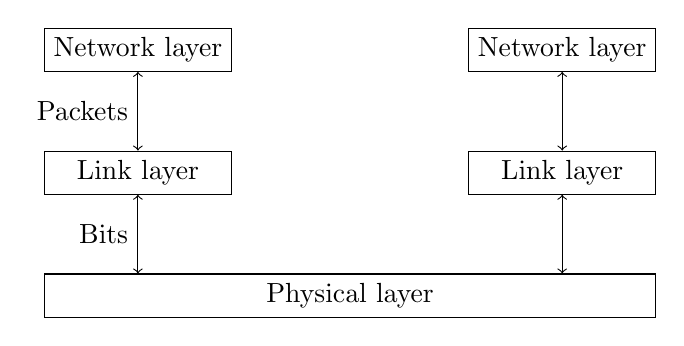
\begin{tikzpicture}
  \label{page:ll:layers}

  \begin{scope}[every node/.style={draw}]
    \node (networkl) {Network layer};
    \node [below=of -(networkl)] (lll) {Link layer};

    \node [right=3cm of networkl] (networkr) {Network layer};
    \node [below=of -(networkr)] (llr) {Link layer};

    \node [below=of -(llr)(lll)] (phy) {Physical layer}; 
  \end{scope}

  \draw [<->] (networkl) to node [left] {Packets} (lll); 
  \draw [<->] (lll) to node [left] {Bits} (lll |- phy.north); 

  \draw [<->] (networkr) -- (llr);
  \draw [<->] (llr) -- (llr |- phy.north); 
  
\end{tikzpicture}


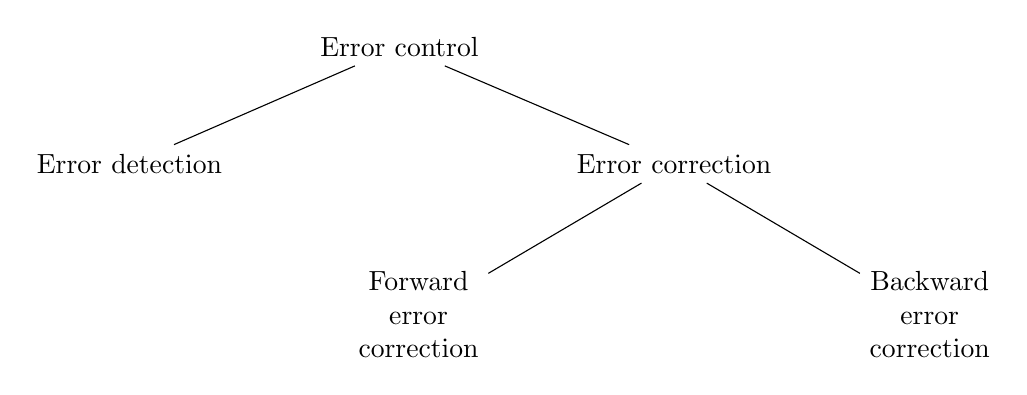
\begin{tikzpicture}
  \label{page:ll:errorcontrol}

  \node (ec) {Error control};
  \node [below left=of ec] (ed) {Error detection};
  \node [below right=of ec] (ecor) {Error correction};
  
  \node [below left=of ecor, align=center] (fwd) {Forward\\ error\\correction};
  \node [below right=of ecor, align=center] (back) {Backward\\error\\correction};

  \draw (ec) edge (ed) -- (ecor) edge (fwd) -- (back);
  
\end{tikzpicture}


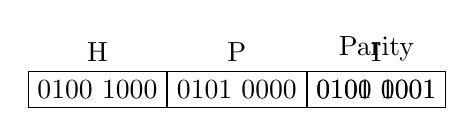
\begin{tikzpicture}
  \label{page:ll:basic_interleaving}

  \begin{scope}[node distance=0, every node/.style={draw}]
    \node[label=above:H] (B1)                   {0100 1000};
    \node[label=above:P, right=of B1] (B2)      {0101 0000};
    \node[label=above:I, right=of B2] (B3)      {0100 1001};
    \node[label=above:Parity, right=of B2] (B3) {0101 0001};
  \end{scope}
\end{tikzpicture}

\end{document}